\clearpage
\phantomsection
\addcontentsline{toc}{chapter}{LAMPIRAN}
\chapter*{LAMPIRAN}

% Reset figure numbering for appendix
\setcounter{figure}{0}
\renewcommand{\thefigure}{L.\arabic{figure}}
\renewcommand{\figurename}{Gambar}
\renewcommand{\cftfigpresnum}{Gambar }
\setlength{\cftfignumwidth}{4.5em}

\section*{Lampiran A: Hasil Pengujian \textit{Code Coverage Backend}}

Lampiran ini menyajikan hasil pengujian \textit{code coverage} \textit{backend} menggunakan \textit{testing framework} Go. Hasil ditampilkan dalam bentuk laporan HTML yang menunjukkan persentase \textit{coverage} dan detail kode yang telah diuji (\textit{covered}) maupun belum diuji (\textit{not covered}).

\subsection*{A.1 Ringkasan \textit{Code Coverage}}

Ringkasan hasil pengujian menunjukkan total \textit{code coverage} sebesar 31,9\%. Modul inti (\textit{auth\_service}, \textit{code\_generator}, \textit{kehadiran\_service}, \textit{peminjaman\_service}) telah mencapai tingkat keterujian tinggi.

\begin{figure}[H]
    \centering
    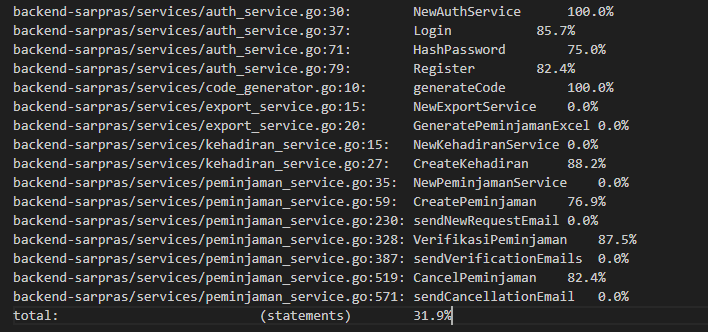
\includegraphics[width=0.9\textwidth]{gambar/media/image25.png}
    \caption{Ringkasan \textit{Code Coverage Backend}}
    \label{fig:coverage_summary}
\end{figure}

\subsection*{A.2 Detail \textit{Coverage}: \textit{Auth Service}}

Detail \textit{coverage} \textit{Auth Service} menunjukkan sebagian besar kode telah tercakup pengujian (hijau), termasuk fungsi kritis seperti \textit{login} dan \textit{register}.

\begin{figure}[H]
    \centering
    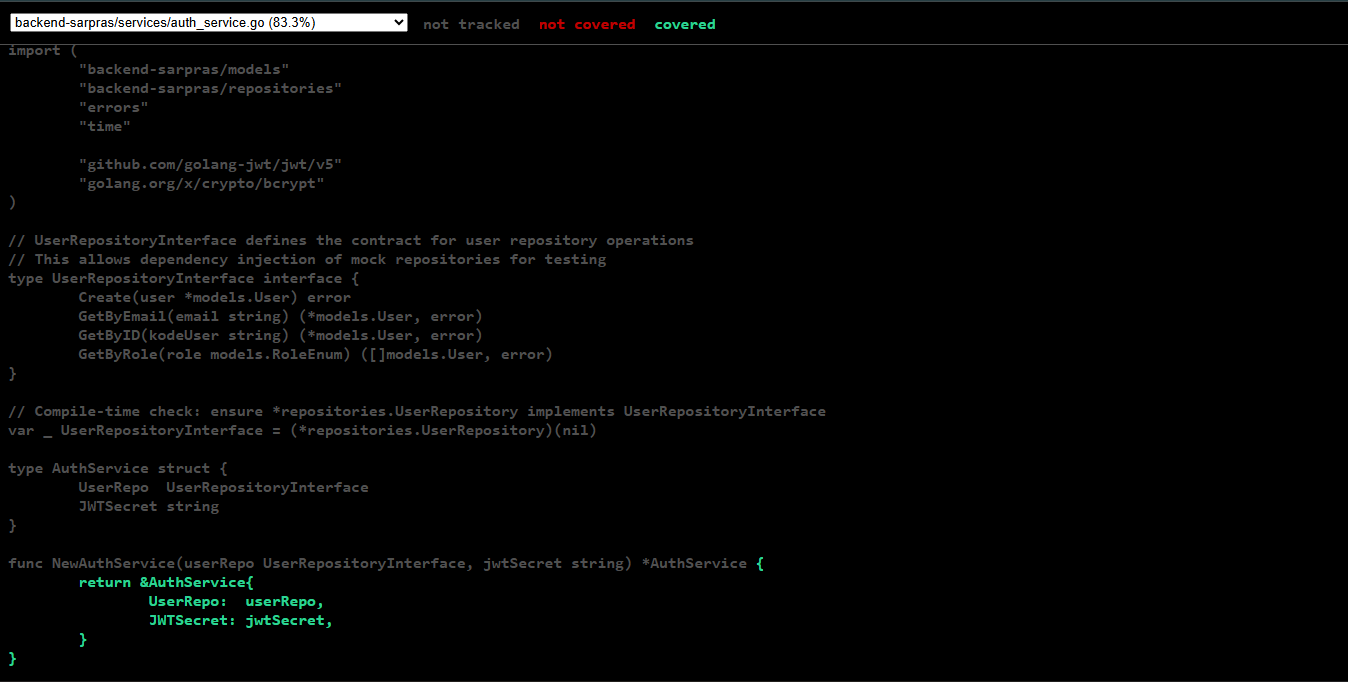
\includegraphics[width=0.9\textwidth]{gambar/media/auth service.png}
    \caption{Detail \textit{Coverage} \textit{Auth Service}}
    \label{fig:coverage_auth}
\end{figure}

\subsection*{A.3 Detail \textit{Coverage}: \textit{Kehadiran Service}}

Detail \textit{coverage} \textit{Kehadiran Service} menunjukkan tingkat \textit{coverage} tinggi (88,2\%), dengan fungsi utama \texttt{CreateKehadiran} telah diuji menyeluruh.

\begin{figure}[H]
    \centering
    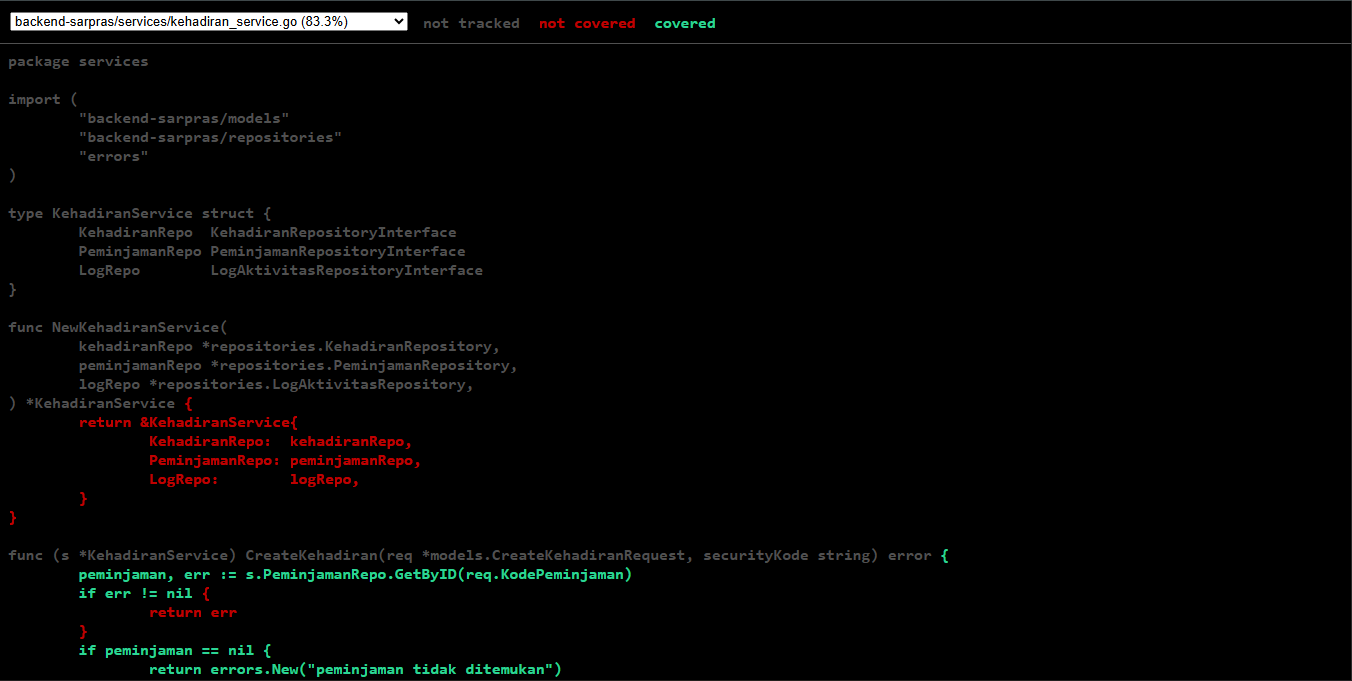
\includegraphics[width=0.9\textwidth]{gambar/media/kehadiran service.png}
    \caption{Detail \textit{Coverage} \textit{Kehadiran Service}}
    \label{fig:coverage_kehadiran}
\end{figure}

\subsection*{A.4 Detail \textit{Coverage}: \textit{Peminjaman Service}}

Detail \textit{coverage} \textit{Peminjaman Service} menunjukkan tingkat \textit{coverage} baik untuk fungsi inti (pengajuan, verifikasi, pembatalan peminjaman).

\begin{figure}[H]
    \centering
    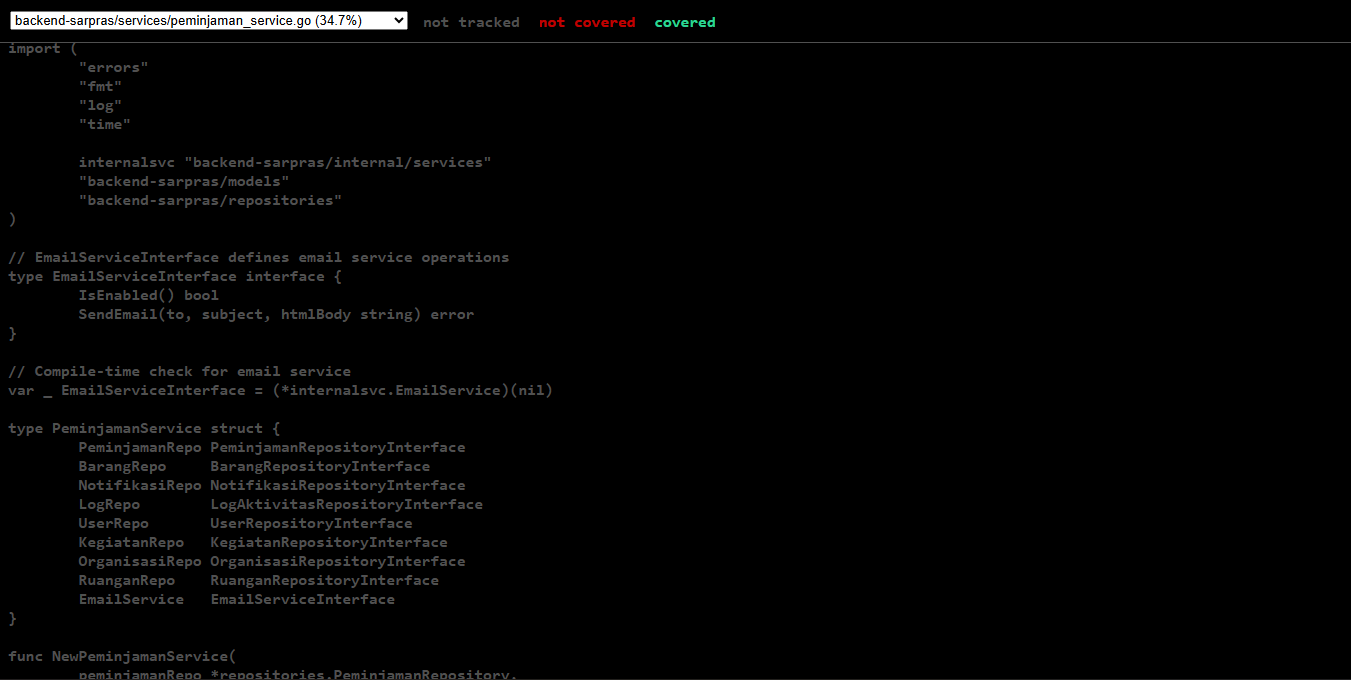
\includegraphics[width=0.9\textwidth]{gambar/media/peminjaman service.png}
    \caption{Detail \textit{Coverage} \textit{Peminjaman Service}}
    \label{fig:coverage_peminjaman}
\end{figure}

\section*{Lampiran B: Dokumentasi Wawancara}

Dokumentasi wawancara dengan staf Sarana dan Prasarana sebagai bagian proses pengumpulan data dan analisis kebutuhan sistem.

\begin{figure}[H]
    \centering
    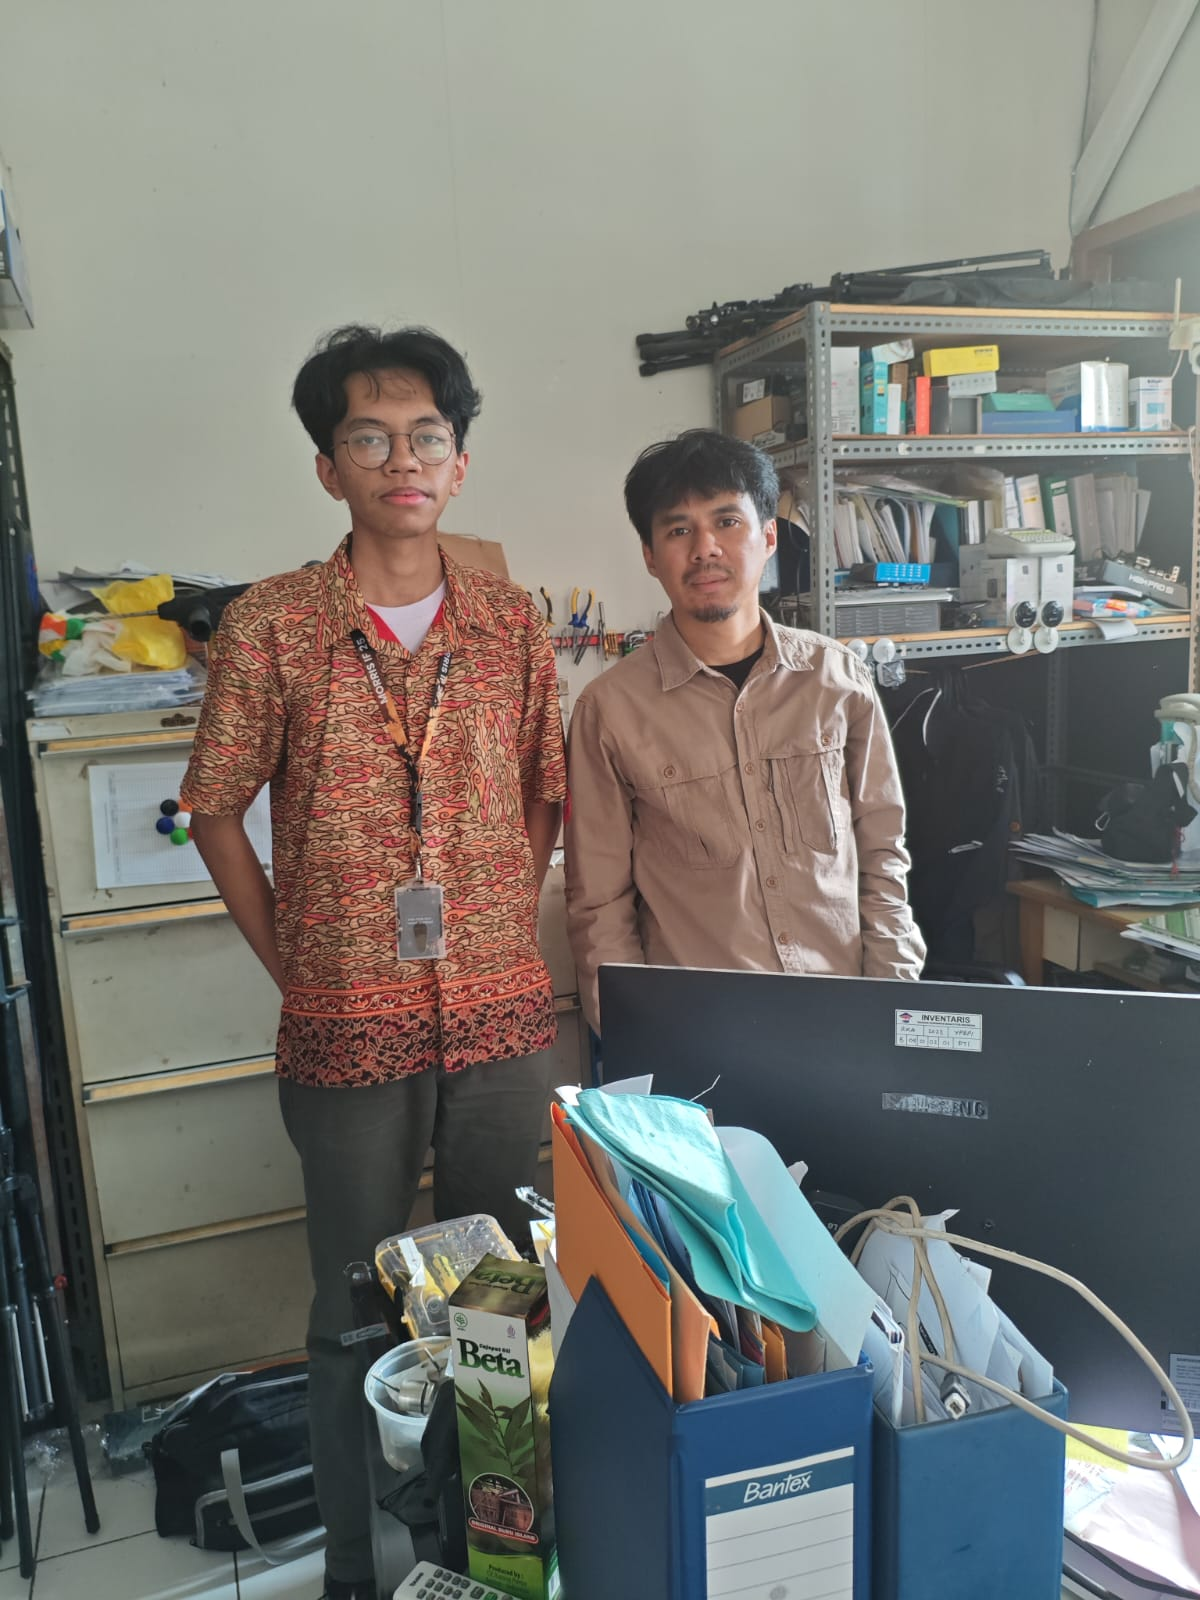
\includegraphics[width=0.5\textwidth]{gambar/media/coblong.jpeg}
    \caption{Dokumentasi Wawancara dengan Staf Sarana dan Prasarana}
    \label{fig:dokumentasi_wawancara}
\end{figure}
